\section{Transmission}

\subsection{Electro-pneumatic Simulation}

The electro-pneumatic Simulink model as described in Sec.\ \ref{sec:electropneumatic_implementation} was simulated by feeding the closed-loop system with a reference input representing 50\% of the maximum travel of the clutch. Figure \ref{fig:pneumatic_sim} shows the closed-loop response to the step input, recorded until the output stabilized. Figure \ref{fig:pneumatic_sim_zoom} shows a close up view of the first peak in the response, detailing the result of the compressibility effects of the air in the cylinder. The PID controller block was minimally tuned only until a stable response was obtained.

\begin{figure}[htp]
 \centering
 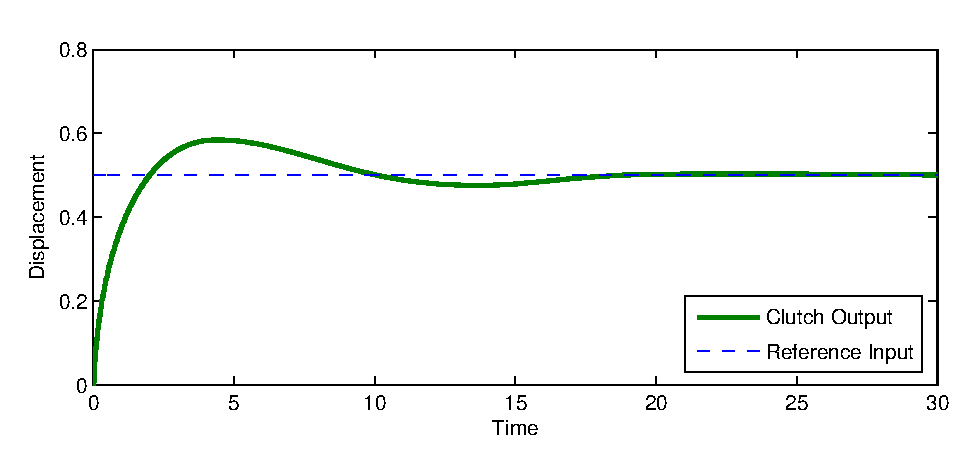
\includegraphics[width=6in,keepaspectratio]{results/figures/electro-pneumatic_simulation_plot.eps}
 \caption{Output from Simulink electro-pneumatic model}
 \label{fig:pneumatic_sim}
\end{figure}

The point of the simulation was to verify the feasability of closed-loop control over the electro-pneumatic system in the configuration proposed. It is important to note that correct model parameters corresponding to the real physical pneumatic valves, cylinders, clutch, etc., were not obtained.

\begin{figure}[htp]
 \centering
 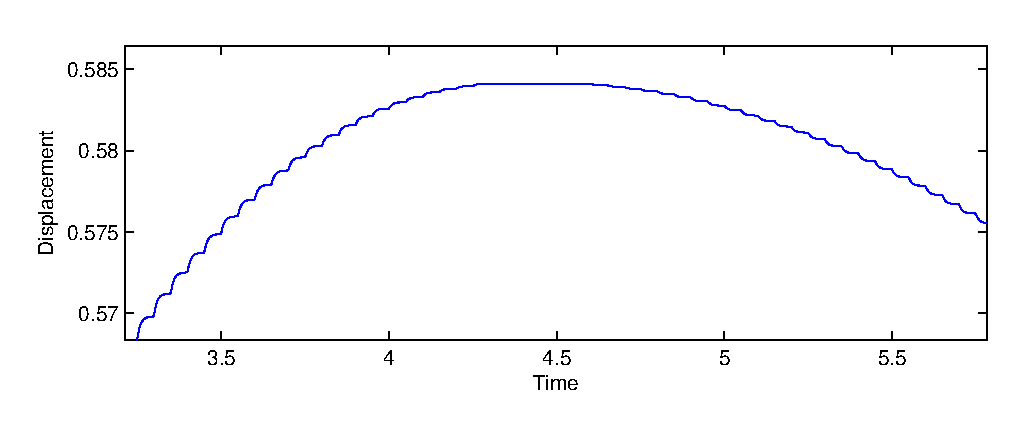
\includegraphics[width=6in,keepaspectratio]{results/figures/electro-pneumatic_simulation_plot2.eps}
 \caption{Close-up of the first peak in Fig. \ref{fig:pneumatic_sim}}
 \label{fig:pneumatic_sim_zoom}
\end{figure}


\subsection{System testing}

Since testing and tuning of the full electro-pneumatic system requires that the 2010 Formula SAE vehicle be complete, this phase of the project was not completed as intended, and is recommended for future work.